As Olimpíadas de Verão Nlogônia 2024 estão sendo um sucesso! Inúmeros atletas
estão em busca da tão sonhada medalha de ouro em diversos esportes.

Um dos esportes disputados é o \textit{arremesso de trinângulo}. Este esporte é
jogado em um campo que pode ser representado em um plano cartesiano. O campo
contém $N$ semicircunferências. Seus raios são $r_1$, $r_2$, ..., $r_N$ em ordem
crescente, todas são centradas na origem, e cada semicircunferência tem seu
\textit{valor} associado.

A figura abaixo exemplifica um campo com $N=3$
semicircunferências, de raios 2, 3 e 5, e valores 2, 1 e 4, respectivamente:

\begin{center}
    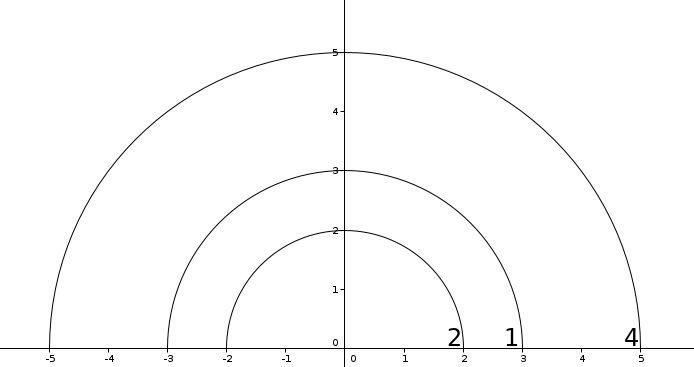
\includegraphics[scale=0.4]{arremesso/campo.png}
\end{center}

Em uma jogada, um atleta arremessa um ponto em uma posição $P$. Em seguida, é
traçado um triângulo cujos vértices são os pontos $P$, $(X_L, 0)$ e $(X_R, 0)$
(os valores de $X_L$ e $X_R$ são definidos pelos juizes). Como exemplo,
considere que um atleta arremessou um ponto na posição $P=(4,5)$, que $X_L = -4$
e $X_R = 1$. A figura abaixo mostra o triângulo traçado:

\begin{center}
    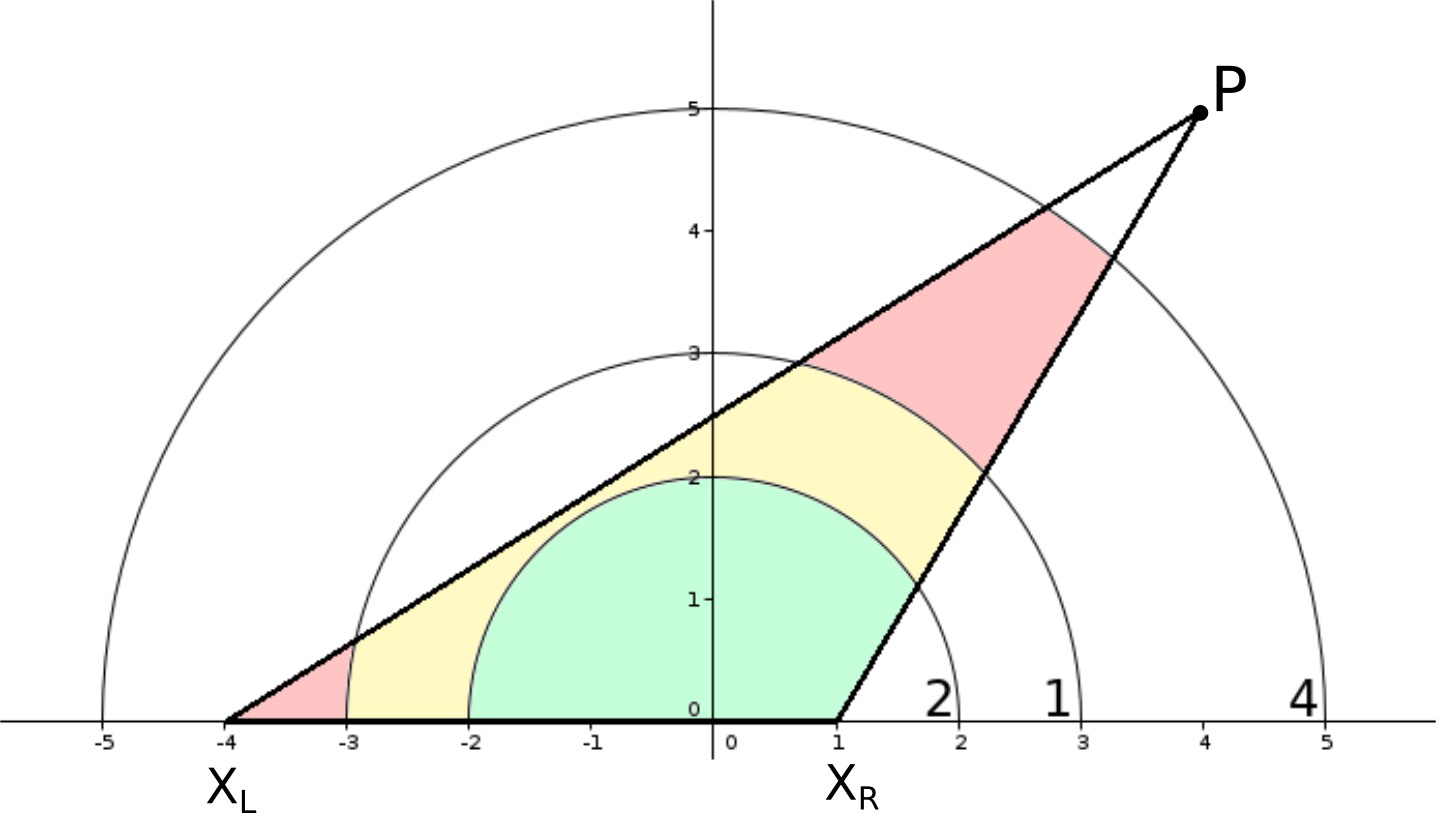
\includegraphics[scale=0.4]{arremesso/score.png}
\end{center}

A \textit{região de pontuação} de uma semicircunferência é a área do seu
semicírculo (no caso da primeira semicircunferência) ou a área entre uma
semicircunferência e a próxima semicircunferência (no caso das demais).

A \textit{pontuação} feita em uma semicircunferência é dada pelo produto entre
seu valor e a área de intersecção entre o triângulo e sua região de pontuação.
A \textit{pontuação total} da jogada é dada pela soma da pontuação feita em
todas as semicircunferências.

No exemplo dado, a pontuação total da jogada será, aproximadamente,
2 $\times$ 5.662733 (a área em verde na figura)
+ 1 $\times$ 3.579953 (a área em amarelo na figura)
+ 4 $\times$ 2.774575 (a área em vermelho na figura)
$\approx$ 26.003719.

Dada a descrição do campo e da jogada, determine sua pontuação total.

\subsection*{Entrada}

A primeira linha contém um inteiro $N$ ($1 \leq N \leq 100$), o número de
semicircunferencias no campo. A próxima linha contém $N$ inteiros $r_i$
$(1 \leq r_i \leq 100)$, os raios das semicircunferências, em ordem crescente.
A próxima linha contém $N$ inteiros $v_i$
$(0 \leq v_i \leq 10$), os valores de cada semicircunferência, na ordem em que são
dados na entrada.
A próxima linha contém dois inteiros $X_L$ e $X_R$
$(-100 \leq X_L \leq 0 \leq X_R \leq 100)$ indicando as coordenadas definidas pelos juizes. A última linha contém dois inteiros
$X_P$ e $Y_P$ ($-100 \leq X_P \leq 100$, $0 \leq Y_P \leq 100$) indicando a
coordenada do ponto arremessado.

Note que tanto os pontos $(X_L,0)$ e $(X_R,0)$ quanto o ponto
$P$ podem ou não estar dentro de algum semi-circulo.

\subsection*{Saída}

Imprima uma única linha contendo a pontuação total da jogada, arredondada com
exatamente duas casas decimais.

%----- Exemplo 1 -----%
\begin{table}[!h]
\centering
\begin{tabular}{|l|l|}
\hline
\begin{minipage}[t]{3in}
\textbf{Exemplo de entrada}
\begin{verbatim}
3
2 3 5
2 1 4
-4 1
4 5
\end{verbatim}
\vspace{1mm}
\end{minipage}
&
\begin{minipage}[t]{3in}
\textbf{Exemplo de saída}
\begin{verbatim}
26.00
\end{verbatim}
\vspace{1mm}
\end{minipage} \\
\hline
\end{tabular}
\end{table}

%----- Exemplo 2 -----%
\begin{table}[!h]
\centering
\begin{tabular}{|l|l|}
\hline
\begin{minipage}[t]{3in}
\textbf{Exemplo de entrada}
\begin{verbatim}
4
1 5 7 8
2 1 0 1
-10 10
0 10
\end{verbatim}
\vspace{1mm}
\end{minipage}
&
\begin{minipage}[t]{3in}
\textbf{Exemplo de saída}
\begin{verbatim}
55.02
\end{verbatim}
\vspace{1mm}
\end{minipage} \\
\hline
\end{tabular}
\end{table}
